
\documentclass[12pt,a4paper]{report}
\usepackage[a4paper,top=2.4cm,bottom=2.4cm,left=2.5cm,right=2.5cm]{geometry}
\usepackage{fontspec}
\setmainfont{Arial}
\usepackage[french]{babel}
\usepackage{graphicx}
\usepackage{pdfpages}
\usepackage{xcolor}
\usepackage{array}
\usepackage{longtable}
\usepackage{booktabs}
\usepackage{enumitem}
\usepackage{hyperref}
\usepackage{fancyhdr}
\usepackage{caption}
\usepackage{float}

\hypersetup{
  colorlinks=true,
  linkcolor=black,
  urlcolor=blue,
  pdftitle={Rapport PFA - Plateforme RH Django},
  pdfauthor={Zine Mohamed Amine et Ghaout Khalid}
}

\setlength{\parindent}{0.7cm}
\setlength{\parskip}{0.25cm}
\setlength{\headheight}{15pt}
\emergencystretch=4em
\renewcommand{\baselinestretch}{1.14}
\setlist[itemize]{topsep=2pt,itemsep=2pt}
\sloppy

\pagestyle{fancy}
\fancyhf{}
\lhead{Plateforme RH Django}
\rhead{\thepage}
\renewcommand{\headrulewidth}{0.2pt}

\begin{document}
\pagenumbering{gobble}
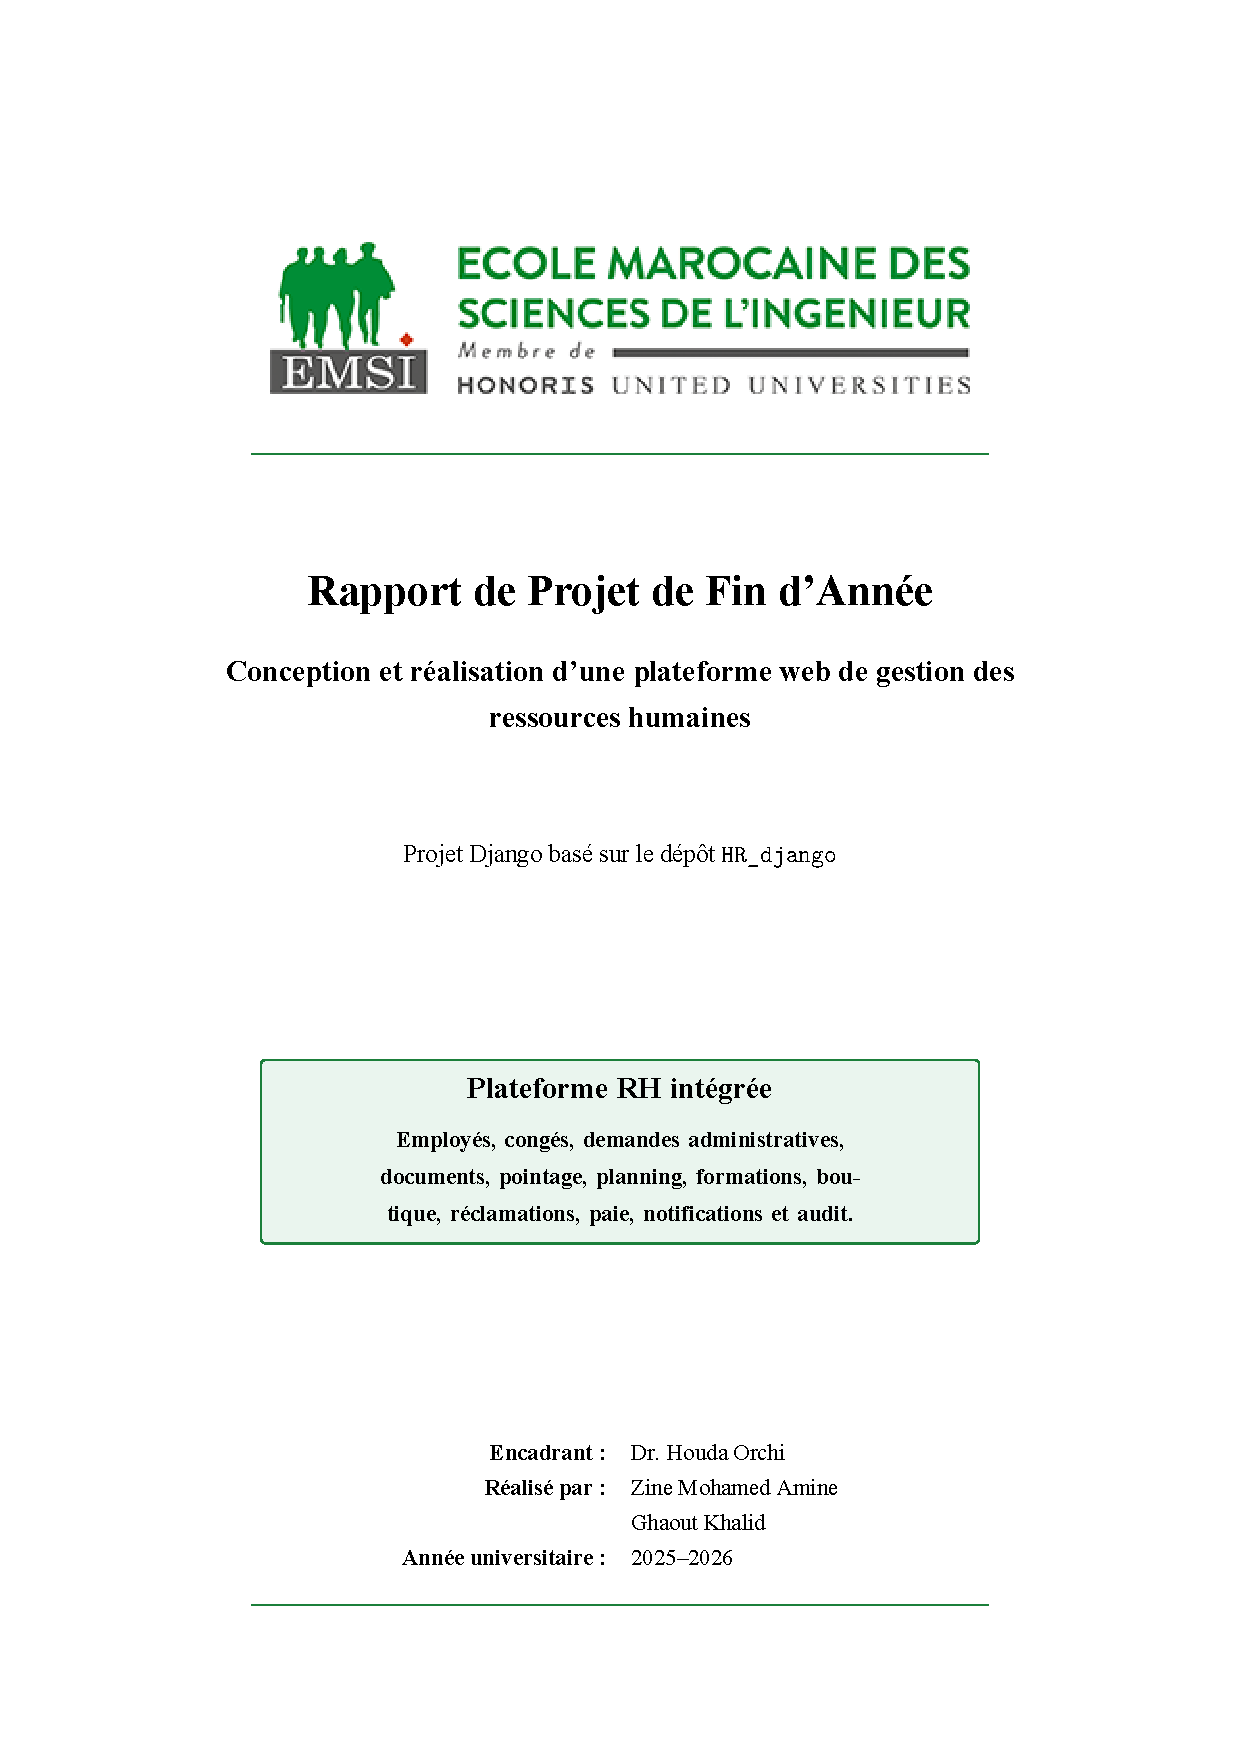
\includepdf[pages=1]{ancienne_page_de_garde.pdf}

\pagenumbering{roman}

\chapter*{Remerciements}
\addcontentsline{toc}{chapter}{Remerciements}
Nous tenons à exprimer notre profonde gratitude à Dr. Houda Orchi pour son encadrement, sa disponibilité et ses conseils tout au long de ce Projet de Fin d'Année. Ses orientations nous ont permis de consolider notre démarche, de mieux organiser l'analyse fonctionnelle et de renforcer la qualité technique de la solution.

Nous remercions également l'ensemble des personnes qui nous ont soutenus durant les phases d'analyse, de conception, de développement, de validation et de rédaction. Leur aide a contribué à transformer l'application RH en une plateforme plus complète, plus cohérente et plus proche des besoins réels d'une organisation.

Enfin, nous adressons nos remerciements à notre établissement et à l'équipe pédagogique pour les connaissances, les méthodes et l'environnement de travail qui ont rendu possible la réalisation de ce projet.
\newpage

\chapter*{Résumé}
\addcontentsline{toc}{chapter}{Résumé}
Ce rapport présente la maintenance, la mise à jour et l'amélioration d'une plateforme web de gestion des ressources humaines développée avec Django. L'application couvre les principaux processus RH : authentification, création de compte, vérification par courriel, réinitialisation du mot de passe, employés, départements, services, postes, congés, demandes administratives, documents, notifications, audit, pointage, planning, tâches d'équipe, support RH sous forme de tickets, formations, actualités, boutique interne, réclamations, points et paie.

La mise à jour majeure concerne le module Planning. Le système prend désormais en charge les shifts normaux, les plans permanents, les règles de récurrence, les pauses, les filtres dynamiques, les vues journalière, hebdomadaire, sur deux semaines et mensuelle, les statistiques, les rapports, la création groupée, la copie de planning, les conflits et les API JSON. Le Planning est relié au module Présence / Pointage afin que les retards, sorties anticipées, heures manquantes et heures supplémentaires soient calculés à partir du shift réellement planifié.

Le projet intègre aussi un assistant intelligent basé sur Gemini. L'assistant général repose sur une approche RAG sécurisée : le backend récupère uniquement le contexte autorisé pour l'utilisateur, refuse les demandes sensibles et utilise un fallback local si l'API n'est pas disponible. L'assistant Planning peut répondre à des questions opérationnelles sur les conflits, les heures planifiées et les employés sans planning. Les actions sensibles restent validées côté backend.

\textbf{Mots-clés :} Django, ressources humaines, planning, pointage, plan permanent, Gemini, RAG, Brevo, sécurité, tickets RH, tâches, audit.
\newpage

\chapter*{Abstract}
\addcontentsline{toc}{chapter}{Abstract}
This report presents the maintenance, update and improvement of a Django-based human resources management platform. The application covers the main HR processes: authentication, account creation, email verification, password reset, employees, departments, services, positions, leave requests, administrative requests, documents, notifications, audit logs, attendance, planning, team tasks, HR support tickets, training, news, internal shop, claims, points and payroll analytics.

The main update concerns the Planning module. The system now supports normal shifts, permanent plans, recurrence rules, breaks, dynamic filters, daily, weekly, biweekly and monthly views, statistics, reports, bulk creation, planning copy, conflict detection and JSON APIs. Planning is connected to Presence / Pointage so that late arrivals, early departures, missing hours and overtime are calculated from the employee's planned shift.

The project also includes a Gemini-powered assistant. The global assistant follows a secure RAG approach: the backend retrieves only the context authorized for the current user, refuses sensitive requests and uses a local fallback when the API is unavailable. The Planning assistant answers operational questions about conflicts, planned hours and employees without planning. Sensitive actions remain validated by the backend.

\textbf{Keywords:} Django, human resources, planning, attendance, permanent plan, Gemini, RAG, Brevo, security, HR tickets, tasks, audit.
\newpage

\listoffigures
\addcontentsline{toc}{chapter}{Liste des figures}
\newpage
\listoftables
\addcontentsline{toc}{chapter}{Liste des tableaux}
\newpage

\chapter*{Liste des abréviations}
\addcontentsline{toc}{chapter}{Liste des abréviations}
\begin{longtable}{p{3cm}p{11cm}}
\toprule
\textbf{Abréviation} & \textbf{Signification}\\
\midrule
API & Application Programming Interface, interface permettant à deux composants logiciels de communiquer.\\
CRUD & Create, Read, Update, Delete, opérations de base sur les données.\\
CSRF & Cross-Site Request Forgery, attaque prévenue par les protections Django.\\
KPI & Key Performance Indicator, indicateur de performance utilisé dans les tableaux de bord.\\
ORM & Object-Relational Mapping, mécanisme Django reliant les objets Python aux tables SQL.\\
RAG & Retrieval-Augmented Generation, génération de réponse enrichie par récupération de contexte.\\
RH & Ressources humaines.\\
UI & User Interface, interface utilisateur.\\
UX & User Experience, expérience utilisateur.\\
WSGI & Web Server Gateway Interface, interface d'exécution Python pour application web.\\
\bottomrule
\end{longtable}
\newpage

\tableofcontents
\newpage

\pagenumbering{arabic}
\setcounter{page}{1}

\chapter*{Introduction générale}
\addcontentsline{toc}{chapter}{Introduction générale}
La gestion des ressources humaines constitue un axe stratégique pour toute organisation moderne. Elle ne se limite plus à l'enregistrement administratif du personnel ; elle couvre également l'organisation interne, les congés, les demandes administratives, la communication RH, la gestion documentaire, la présence, la planification, les tâches, la formation, les réclamations, les points, la paie et l'audit. Dans un environnement où les données sont sensibles et nombreuses, une gestion manuelle ou dispersée entraîne des erreurs, des retards et une faible traçabilité.

Le projet étudié est une plateforme RH développée avec Django. Le dépôt courant contient trois grandes applications : \texttt{accounts}, qui gère les rôles, les profils, les demandes de compte, la vérification de courriel et la réinitialisation du mot de passe ; \texttt{core}, qui porte le tableau de bord, l'administration et l'assistant global ; et \texttt{hr}, qui regroupe les modèles métier, formulaires, vues, services, permissions, templates, tests et commandes de données de démonstration.

La version finale de l'application apporte plusieurs évolutions importantes par rapport au rapport initial. Les anciennes intégrations décrites dans la première version sont remplacées par une intégration Gemini et Brevo. Le module Planning est fortement enrichi : il gère les plans normaux, les plans permanents, les récurrences, les pauses, les vues calendrier, les statistiques, les rapports, les conflits, les API et l'assistant spécialisé. Le pointage utilise désormais le shift planifié comme référence de calcul. Le support RH devient un système de tickets avec clôture, participants, pièces jointes, notes et évaluation. L'administration intègre les demandes de création de compte, les paramètres de sécurité, les modèles Brevo, l'audit et les décisions d'approbation.

La problématique de ce travail peut être formulée ainsi : comment maintenir et améliorer une plateforme RH Django existante afin qu'elle corresponde à l'état réel de l'application, respecte les règles de sécurité et fournisse un rapport technique conforme aux consignes académiques ? Pour répondre à cette problématique, la démarche adoptée consiste à utiliser le code source courant comme source de vérité, à conserver les éléments encore corrects de l'ancien rapport, à supprimer les références obsolètes et à documenter les modules ajoutés ou transformés.

Ce rapport est organisé en quatre chapitres. Le premier chapitre présente le contexte général du projet, la problématique, les objectifs, l'étude de l'existant et la méthodologie adoptée. Le deuxième chapitre analyse les acteurs, les besoins fonctionnels, les besoins non fonctionnels et les principaux cas d'utilisation. Le troisième chapitre expose la conception, l'architecture, le modèle de données, les diagrammes de séquence et les choix technologiques. Le quatrième chapitre présente la réalisation, les interfaces, les tests, la validation, le déploiement et les difficultés rencontrées. Le rapport se termine par une conclusion générale et des annexes.

\chapter{Présentation générale du projet}
\section{Introduction}
Ce chapitre situe le projet dans son contexte fonctionnel et technique. Il présente les limites de l'existant, les objectifs de la solution, les améliorations apportées à l'application et la méthodologie suivie. Il permet aussi de comprendre pourquoi le rapport devait être mis à jour : plusieurs fonctionnalités importantes ont évolué après la première version, notamment le Planning, le Pointage, l'Administration, le support RH, les comptes utilisateurs et l'assistant.

\section{Contexte général}
La plateforme RH Django est une application web interne destinée à centraliser les opérations de gestion des ressources humaines. Elle fournit un espace unique pour les employés, les responsables hiérarchiques, les responsables RH et les administrateurs. Chaque profil possède un accès différent selon son rôle.

L'application repose sur une architecture Django classique : configuration dans \texttt{config}, authentification et profils dans \texttt{accounts}, tableau de bord et administration dans \texttt{core}, logique RH dans \texttt{hr}, templates dans \texttt{templates}, fichiers statiques dans \texttt{static} et médias dans \texttt{media}. Cette organisation permet de séparer les responsabilités et de faire évoluer les modules sans mélanger l'interface, les règles métier et la persistance.

La version actuelle ne se limite pas aux fonctionnalités initiales. Elle comprend désormais un workflow complet de création de compte avec vérification par code, un workflow de mot de passe oublié, des paramètres administratifs Brevo, un assistant Gemini, un Planning évolué, des tickets RH, des tâches d'équipe avec points, un arbre hiérarchique et une administration plus structurée.

\section{Problématique}
Les processus RH doivent être fiables, confidentiels et traçables. Une erreur de solde, une fuite de données personnelles, une planification incohérente ou un pointage mal calculé peut produire des conséquences importantes sur la qualité de service et sur la confiance des utilisateurs.

La difficulté principale consiste donc à construire une application qui centralise les données tout en respectant le périmètre de chaque rôle. Un employé ne doit consulter que ses informations. Un manager doit accéder à son équipe sans voir toute l'entreprise. Un responsable RH ou administrateur doit pouvoir traiter les workflows sensibles, mais ces actions doivent rester validées, auditées et protégées.

La deuxième difficulté concerne la cohérence entre Planning et Pointage. Le calcul de présence ne peut pas être fiable si l'on se base uniquement sur une heure officielle globale. La version actuelle résout cette limite en associant le pointage au shift planifié, puis en calculant les écarts entre le prévu et le réel.

\section{Étude de l'existant}
La première version du rapport décrivait déjà une plateforme RH large, mais certaines informations sont devenues obsolètes. Les anciennes références IA doivent être remplacées par Gemini. Les descriptions de messagerie RH doivent être remplacées par le système de tickets actuel. Les workflows de création de compte et de réinitialisation du mot de passe doivent intégrer la vérification par code et Brevo. Le Planning doit être décrit comme un module complet, et non comme une simple liste de shifts.

L'existant manuel ou semi-numérique présente aussi des limites classiques : fichiers dispersés, validations non tracées, absence d'historique, dépendance à la mémoire des acteurs, faible visibilité sur les présences, difficulté à gérer les plannings récurrents et impossibilité de répondre rapidement aux questions des utilisateurs.


\begin{longtable}{>{\raggedright\arraybackslash}p{4cm}>{\raggedright\arraybackslash}p{4cm}>{\raggedright\arraybackslash}p{6cm}}
\caption{Critique de l'existant et réponse apportée}\label{tab:critique-existant}\\
\toprule
\textbf{Limite} & \textbf{Risque} & \textbf{Réponse actuelle} \\
\midrule
\endfirsthead
\toprule
\textbf{Limite} & \textbf{Risque} & \textbf{Réponse actuelle} \\
\midrule
\endhead
Données RH dispersées & Perte d'information et doublons & Centralisation dans les modèles Django et affichage par rôle. \\
Validation manuelle & Décisions non tracées & Workflows backend, notifications et historique d'audit. \\
Pointage indépendant du planning & Calculs de présence imprécis & Lien direct entre \texttt{Pointage} et \texttt{PlanningShift}. \\
Planning non permanent & Répétition manuelle des horaires standards & Plans permanents avec heure de fin standard et règles de récurrence. \\
Assistance non sécurisée & Risque de fuite d'informations & RAG avec contexte autorisé, refus de sécurité et Gemini optionnel. \\
Création de compte manuelle & Comptes créés sans vérification & Demande de compte, code Brevo, approbation administrateur et onboarding RH. \\
\bottomrule
\end{longtable}


\section{Objectifs du projet}
Les objectifs principaux sont les suivants :
\begin{itemize}
\item centraliser les données et workflows RH dans une application unique ;
\item sécuriser les accès selon les rôles administrateur, responsable RH, responsable hiérarchique et employé ;
\item mettre à jour la documentation pour remplacer les références obsolètes par l'implémentation actuelle ;
\item décrire le Planning comme un module complet de planification opérationnelle ;
\item relier clairement le Planning au Pointage pour expliquer les calculs de présence ;
\item documenter la création de compte, la vérification courriel, l'approbation administrateur et le mot de passe oublié ;
\item présenter l'assistant Gemini et son fonctionnement RAG sécurisé ;
\item conserver une structure de rapport conforme aux consignes académiques.
\end{itemize}


\section{Méthodologie adoptée}
La démarche suivie est une démarche de maintenance documentaire guidée par le code source. Le code courant est considéré comme la source de vérité. Les sections correctes de l'ancien rapport sont conservées dans leur logique et leur style, tandis que les sections devenues inexactes sont modifiées. Les fonctionnalités ajoutées sont intégrées dans les chapitres appropriés.

La vérification technique repose sur l'inspection des modèles, vues, services, formulaires, templates, routes et tests. Les tests ciblés du Planning, de l'assistant et des workflows de compte ont été utilisés comme preuves de comportement. Les règles de rapport du superviseur ont ensuite été contrôlées : introduction générale non numérotée, conclusion générale non numérotée, chapitres avec introduction et conclusion, listes obligatoires et numérotation des figures et tableaux par chapitre.

\section{Planning prévisionnel}

\begin{longtable}{>{\raggedright\arraybackslash}p{4cm}>{\raggedright\arraybackslash}p{10cm}}
\caption{Planning prévisionnel du projet}\label{tab:planning-previsionnel}\\
\toprule
\textbf{Phase} & \textbf{Travaux réalisés} \\
\midrule
\endfirsthead
\toprule
\textbf{Phase} & \textbf{Travaux réalisés} \\
\midrule
\endhead
Analyse & Lecture du code source, du PDF existant, des règles de rapport et du prompt de maintenance documentaire. \\
Audit & Identification des références obsolètes : ancienne solution IA, anciennes explications de messagerie, anciens workflows de compte. \\
Conception documentaire & Mise à jour de l'architecture, des cas d'utilisation, des diagrammes et du dictionnaire de données. \\
Rédaction & Ajout des modules Planning, Pointage, Gemini, Brevo, Administration, Tickets RH et Tâches. \\
Validation & Compilation LaTeX, contrôles de structure et tests Django ciblés. \\
\bottomrule
\end{longtable}


\section{Conclusion}
Ce chapitre a présenté le contexte, la problématique, les limites de l'existant et la méthode retenue pour maintenir le rapport. La suite du document précise les besoins fonctionnels et non fonctionnels de la plateforme actuelle.

\chapter{Analyse et spécification des besoins}
\section{Introduction}
Ce chapitre décrit les acteurs, les besoins fonctionnels, les besoins non fonctionnels et les principaux cas d'utilisation. Les besoins sont formulés à partir du code courant et non à partir d'une version ancienne de l'application.

\section{Acteurs du système}

\begin{longtable}{>{\raggedright\arraybackslash}p{3cm}>{\raggedright\arraybackslash}p{5cm}>{\raggedright\arraybackslash}p{6cm}}
\caption{Acteurs du système}\label{tab:acteurs}\\
\toprule
\textbf{Acteur} & \textbf{Responsabilité} & \textbf{Accès principal} \\
\midrule
\endfirsthead
\toprule
\textbf{Acteur} & \textbf{Responsabilité} & \textbf{Accès principal} \\
\midrule
\endhead
Administrateur & Supervision et sécurité & Administration, demandes de compte, audit, paramètres, paie, utilisateurs. \\
Responsable RH & Gestion opérationnelle RH & Employés, congés, demandes, documents, planning, tickets, formations, réclamations. \\
Responsable hiérarchique & Suivi d'équipe & Collaborateurs directs, planning visible, pointages, tâches, demandes liées au périmètre. \\
Employé & Utilisation personnelle & Profil, planning personnel, pointage, demandes, tickets RH, formations, boutique. \\
Assistant Gemini & Aide contrôlée & Réponses basées sur le contexte autorisé ; aucune écriture directe en base. \\
\bottomrule
\end{longtable}


\section{Besoins fonctionnels}
La plateforme doit permettre l'authentification et la gestion des profils. Le modèle \texttt{UtilisateurProfile} porte le rôle, l'état actif et le lien vers l'employé. Les utilisateurs peuvent demander un compte via un formulaire public. Le système envoie un code de vérification par courriel, place la demande en attente après validation du code, puis laisse l'administrateur approuver ou refuser la demande.

Le workflow de mot de passe oublié doit permettre à un utilisateur de demander un code, de vérifier ce code et de définir un nouveau mot de passe. Les codes sont hachés, limités en nombre de tentatives, soumis à expiration et à cooldown de renvoi.

Le module Employés doit gérer les informations personnelles, l'organisation interne, les postes, les niveaux, les responsables et l'arbre hiérarchique. Les validations empêchent les matricules ou courriels en doublon, les dates incohérentes et les boucles hiérarchiques.

Le module Planning doit gérer des shifts normaux, des plans permanents, des pauses, des récurrences, des conflits, des filtres, des vues calendrier, des statistiques, des rapports, des API et un assistant spécialisé. Il doit rester relié au pointage.

Le module Présence / Pointage doit permettre l'entrée et la sortie du jour, empêcher les doublons, calculer les heures, les retards, les sorties anticipées, les heures manquantes, les heures supplémentaires et les points.

Le support RH doit fonctionner comme un système de tickets : sujet, catégorie, priorité, participants, responsable RH, statut, pièces jointes, clôture, motif de clôture, note de satisfaction et historique des messages.

Le module Tâches d'équipe doit permettre au manager de créer des tâches directes, ouvertes ou d'équipe, de suivre les statuts, de demander des changements, d'archiver, d'attribuer des points et de lier une tâche à un shift.


\begin{longtable}{>{\raggedright\arraybackslash}p{3.5cm}>{\raggedright\arraybackslash}p{10.5cm}}
\caption{Synthèse des besoins fonctionnels}\label{tab:besoins-fonctionnels}\\
\toprule
\textbf{Module} & \textbf{Besoins} \\
\midrule
\endfirsthead
\toprule
\textbf{Module} & \textbf{Besoins} \\
\midrule
\endhead
Comptes & Demande de compte, vérification courriel, approbation administrateur, onboarding RH. \\
Sécurité & Connexion, profil actif, rôles, refus des accès directs non autorisés. \\
Administration & Demandes de compte, utilisateurs, permissions, audit, paramètres Brevo et sécurité. \\
Employés & CRUD, archivage, organisation, postes, niveaux, hiérarchie et arbre. \\
Planning & Plans normaux, plans permanents, récurrence, pauses, conflits, rapports et API. \\
Pointage & Entrée, sortie, shift associé, retards, sorties anticipées, heures manquantes, points. \\
Tickets RH & Conversation, affectation, participants, pièces jointes, clôture, notation. \\
Tâches & Affectation directe, tâches ouvertes, workflow manager, points, archives. \\
Assistant & RAG sécurisé, Gemini, fallback local, refus des mutations dangereuses. \\
\bottomrule
\end{longtable}


\section{Besoins non fonctionnels}
\begin{itemize}
\item Sécurité : les vues sensibles doivent être protégées par authentification et contrôle de rôle.
\item Confidentialité : les querysets doivent filtrer les données selon le profil connecté.
\item Traçabilité : les actions importantes doivent être enregistrées dans l'historique.
\item Robustesse : les validations doivent être présentes côté modèle, formulaire ou service.
\item Ergonomie : les écrans doivent être lisibles, compacts, responsives et cohérents.
\item Maintenabilité : la logique critique doit rester dans les services et non dans les templates.
\item Interopérabilité : les API Planning doivent retourner des réponses JSON homogènes.
\item Résilience IA : l'assistant doit fonctionner en fallback si Gemini est indisponible.
\end{itemize}


\section{Diagramme global des cas d'utilisation}

\begin{figure}[h!]
\centering
\renewcommand{\arraystretch}{1.25}
\begin{tabular}{|>{\centering\arraybackslash}p{4cm}|>{\centering\arraybackslash}p{10cm}|}
\hline
Employé & Pointer, consulter son planning, soumettre des demandes, créer un ticket RH, suivre ses formations \\ \hline
Manager & Consulter son équipe, suivre les tâches, vérifier les présences et les plannings visibles \\ \hline
Responsable RH & Gérer employés, congés, tickets, formations, documents, réclamations et planning \\ \hline
Administrateur & Approuver comptes, gérer paramètres, consulter audit, gérer paie et sécurité \\ \hline
Assistant Gemini & Répondre avec contexte autorisé, refuser les demandes hors périmètre \\ \hline
\end{tabular}
\caption{Diagramme global des cas d'utilisation}
\label{fig:use-cases}
\end{figure}


\section{Description des principaux cas d'utilisation}

\begin{longtable}{>{\raggedright\arraybackslash}p{4cm}>{\raggedright\arraybackslash}p{10cm}}
\caption{Cas d'utilisation : demande de création de compte}\label{tab:cu-compte}\\
\toprule
\textbf{Élément} & \textbf{Description} \\
\midrule
\endfirsthead
\toprule
\textbf{Élément} & \textbf{Description} \\
\midrule
\endhead
Acteur & Visiteur souhaitant obtenir un compte. \\
Objectif & Créer une demande de compte vérifiée par courriel puis approuvée par l'administrateur. \\
Préconditions & Courriel autorisé, mot de passe conforme, aucune demande active en doublon. \\
Scénario nominal & Le visiteur remplit le formulaire, reçoit un code Brevo, vérifie le code, puis attend la décision administrateur. \\
Postconditions & Un compte utilisateur et une tâche d'onboarding RH sont créés après approbation. \\
\bottomrule
\end{longtable}

\begin{longtable}{>{\raggedright\arraybackslash}p{4cm}>{\raggedright\arraybackslash}p{10cm}}
\caption{Cas d'utilisation : création d'un planning}\label{tab:cu-planning}\\
\toprule
\textbf{Élément} & \textbf{Description} \\
\midrule
\endfirsthead
\toprule
\textbf{Élément} & \textbf{Description} \\
\midrule
\endhead
Acteur & Responsable RH ou administrateur. \\
Objectif & Créer un shift normal ou un plan permanent. \\
Préconditions & Rôle autorisé, dates valides, employé actif, absence de conflit. \\
Scénario nominal & L'acteur saisit les horaires, la pause, la cible, le type et le statut. Le service valide puis sauvegarde. \\
Alternatives & Chevauchement, congé validé, pause invalide ou plan permanent déjà actif : création refusée. \\
\bottomrule
\end{longtable}

\begin{longtable}{>{\raggedright\arraybackslash}p{4cm}>{\raggedright\arraybackslash}p{10cm}}
\caption{Cas d'utilisation : pointage fondé sur le planning}\label{tab:cu-pointage}\\
\toprule
\textbf{Élément} & \textbf{Description} \\
\midrule
\endfirsthead
\toprule
\textbf{Élément} & \textbf{Description} \\
\midrule
\endhead
Acteur & Employé. \\
Objectif & Enregistrer la présence et calculer les écarts avec le shift prévu. \\
Préconditions & Profil employé actif et aucun pointage déjà ouvert. \\
Scénario nominal & L'entrée associe le shift planifié ; la sortie calcule heures, retard, sortie anticipée, manque horaire et points. \\
Alternative & Si aucun shift n'existe, un avertissement est affiché et les heures manquantes ne sont pas inventées. \\
\bottomrule
\end{longtable}


\section{Conclusion}
Ce chapitre a formalisé les besoins de la version actuelle de la plateforme. Les besoins montrent que l'application dépasse le cadre d'un simple CRUD RH : elle inclut des workflows de sécurité, un planning opérationnel, une présence calculée, des tickets RH, des tâches d'équipe et un assistant intelligent contrôlé.

\chapter{Conception et choix technologiques}
\section{Introduction}
Ce chapitre présente l'architecture, le modèle de données, les diagrammes de séquence, le modèle relationnel et les choix technologiques. Il remplace les descriptions obsolètes par l'architecture réelle observée dans le code.

\section{Architecture applicative}
L'architecture suit une séparation en couches. Les templates affichent les données et déclenchent les actions. Les vues récupèrent le profil utilisateur, appliquent les permissions et appellent les services. Les services portent les traitements métier : planning, pointage, transactions de points, notifications, audit, courriels Brevo et assistant. Les modèles Django définissent les entités et leurs validations.


\begin{figure}[h!]
\centering
\renewcommand{\arraystretch}{1.25}
\begin{tabular}{|>{\centering\arraybackslash}p{4cm}|>{\centering\arraybackslash}p{10cm}|}
\hline
Interface & Templates Django, Bootstrap, CSS, JavaScript, modals, offcanvas, widgets assistant \\ \hline
Vues & accounts.views, core.views, hr.views \\ \hline
Services & accounts.services, hr.services, hr.planning\_services, hr.planning\_assistant, core.ai\_assistant \\ \hline
Données & Modèles Django, migrations, SQLite local \\ \hline
Externes & Gemini via google-genai, Brevo via API courriel \\ \hline
\end{tabular}
\caption{Architecture applicative en couches}
\label{fig:architecture}
\end{figure}


\section{Modèle de données et diagramme de classes}
Le modèle de données s'appuie sur des entités dédiées aux comptes, à l'organisation RH, au planning, au pointage, aux tickets, aux tâches, à l'audit et aux points. Le diagramme suivant synthétise les classes métier les plus structurantes.


\begin{figure}[h!]
\centering
\renewcommand{\arraystretch}{1.25}
\begin{tabular}{|>{\centering\arraybackslash}p{4cm}|>{\centering\arraybackslash}p{10cm}|}
\hline
UtilisateurProfile & user, role, actif, employe \\ \hline
AccountCreation\newline Request & email, status, email\_verified, employee, user, onboarding\_task \\ \hline
VerificationCode & email, purpose, code\_hash, expires\_at, attempts \\ \hline
Employe & matricule, nom, prenom, departement, service, poste, responsable \\ \hline
PlanningShift & plan\_type, recurrence\_rule, date\_debut, date\_fin, pause, statut \\ \hline
Pointage & shift, heure\_entree, heure\_sortie, total\_heures, statut, points\_calcules \\ \hline
ConversationRH & numero\_ticket, categorie, priorite, statut, responsable\_rh, participants, note \\ \hline
TacheEquipe & mode\_affectation, statut, manager, shift, points\_attribues \\ \hline
\end{tabular}
\caption{Diagramme de classes métier synthétique}
\label{fig:classes}
\end{figure}



\begin{longtable}{>{\raggedright\arraybackslash}p{3.5cm}>{\raggedright\arraybackslash}p{5cm}>{\raggedright\arraybackslash}p{5.5cm}}
\caption{Dictionnaire de données synthétique}\label{tab:dictionnaire}\\
\toprule
\textbf{Entité} & \textbf{Attributs clés} & \textbf{Rôle} \\
\midrule
\endfirsthead
\toprule
\textbf{Entité} & \textbf{Attributs clés} & \textbf{Rôle} \\
\midrule
\endhead
UtilisateurProfile & role, actif, employe & Porte les droits applicatifs. \\
AccountCreation\newline Request & email, status, password\_hash & Gère le cycle de demande de compte. \\
VerificationCode & purpose, code\_hash, expires\_at & Sécurise les vérifications par code. \\
Employe & matricule, organisation, responsable & Pivot métier RH. \\
PlanningShift & dates, type, récurrence, pause & Planifie les shifts et plans permanents. \\
Pointage & shift, entrée, sortie, statut & Calcule la présence réelle. \\
ConversationRH & ticket, statut, priorité, note & Support RH sous forme de ticket. \\
TacheEquipe & mode, statut, points & Suivi opérationnel manager. \\
HistoriqueAction & action, détails, utilisateur & Audit des actions sensibles. \\
\bottomrule
\end{longtable}


\section{Diagrammes de séquence}

\begin{figure}[h!]
\centering
\renewcommand{\arraystretch}{1.25}
\begin{tabular}{|>{\centering\arraybackslash}p{1.5cm}|>{\centering\arraybackslash}p{12.5cm}|}
\hline
1 & Le visiteur soumet le formulaire de création de compte. \\ \hline
2 & AccountRequestService crée la demande et génère un code de vérification. \\ \hline
3 & BrevoEmailService envoie le code de vérification. \\ \hline
4 & Le visiteur saisit le code ; le statut passe à pending. \\ \hline
5 & L'administrateur approuve ; le compte utilisateur et l'onboarding RH sont créés. \\ \hline
\end{tabular}
\caption{Séquence de demande de compte et approbation}
\label{fig:sequence-compte}
\end{figure}

\begin{figure}[h!]
\centering
\renewcommand{\arraystretch}{1.25}
\begin{tabular}{|>{\centering\arraybackslash}p{1.5cm}|>{\centering\arraybackslash}p{12.5cm}|}
\hline
1 & RH/Admin crée un PlanningShift normal ou permanent. \\ \hline
2 & Le modèle valide les dates, la pause, les conflits et les congés. \\ \hline
3 & L'employé pointe l'entrée ; le service recherche le shift applicable. \\ \hline
4 & La sortie calcule les écarts par rapport à la fenêtre planifiée. \\ \hline
5 & Les points et le commentaire de présence sont enregistrés. \\ \hline
\end{tabular}
\caption{Séquence Planning vers Pointage}
\label{fig:sequence-planning-pointage}
\end{figure}

\begin{figure}[h!]
\centering
\renewcommand{\arraystretch}{1.25}
\begin{tabular}{|>{\centering\arraybackslash}p{1.5cm}|>{\centering\arraybackslash}p{12.5cm}|}
\hline
1 & L'utilisateur envoie une question. \\ \hline
2 & Le backend identifie le rôle et refuse les demandes dangereuses. \\ \hline
3 & Les retrievers récupèrent uniquement les données autorisées. \\ \hline
4 & Gemini reçoit un prompt borné ; si indisponible, fallback local. \\ \hline
5 & La réponse retourne sources et actions de navigation autorisées. \\ \hline
\end{tabular}
\caption{Séquence de l'assistant Gemini sécurisé}
\label{fig:sequence-gemini}
\end{figure}


\section{Choix technologiques}

\begin{longtable}{>{\raggedright\arraybackslash}p{3.5cm}>{\raggedright\arraybackslash}p{4cm}>{\raggedright\arraybackslash}p{6.5cm}}
\caption{Choix technologiques et justification}\label{tab:technos}\\
\toprule
\textbf{Technologie} & \textbf{Utilisation} & \textbf{Justification} \\
\midrule
\endfirsthead
\toprule
\textbf{Technologie} & \textbf{Utilisation} & \textbf{Justification} \\
\midrule
\endhead
Python 3.12 & Langage & Lisible, adapté aux projets Django et aux scripts de seed. \\
Django 5.0.6 & Framework web & ORM, vues, templates, sécurité, formulaires, tests. \\
SQLite & Base locale & Suffisant pour développement et démonstration. \\
Bootstrap 5.3 & Interface & Composants responsive et cohérents. \\
Bootstrap Icons & Icônes & Lecture rapide des actions et statuts. \\
google-genai & Gemini & Assistant intelligent configuré par variables d'environnement. \\
Brevo & Courriel & Vérification de compte et mot de passe oublié. \\
MiKTeX/XeLaTeX & Rapport & Compilation PDF avec accents français et page de garde conservée. \\
\bottomrule
\end{longtable}


\section{Conclusion}
La conception met en évidence une architecture modulaire : comptes et sécurité dans \texttt{accounts}, pilotage et assistant dans \texttt{core}, logique RH dans \texttt{hr}. Les diagrammes actualisés remplacent les anciens workflows obsolètes et décrivent les modules réels de la version finale.

\chapter{Réalisation, tests, validation et déploiement}
\section{Introduction}
Ce chapitre présente l'environnement, les modules réalisés, les tests, le déploiement et les difficultés rencontrées. Il met l'accent sur les fonctionnalités ajoutées après la première version du rapport.

\section{Environnement de développement}
Le projet est exécuté localement sous Windows avec Python 3.12.10, Django 5.0.6, SQLite, Bootstrap, Pillow et google-genai. La configuration utilise le fuseau horaire \texttt{Africa/Casablanca}, les fichiers statiques dans \texttt{static} et les médias dans \texttt{media}. Les clés sensibles sont lues depuis les variables d'environnement.

\section{Authentification, comptes et Brevo}
Le système de compte a été renforcé. La page de connexion propose désormais la demande de création de compte et le mot de passe oublié. Une demande de compte passe par un code de vérification. Le code est haché, limité en durée et en tentatives. Après vérification du courriel, l'administrateur décide d'approuver ou de refuser. En cas d'approbation, le compte utilisateur est créé et une tâche d'onboarding RH peut être générée.

Le mot de passe oublié suit une logique similaire : demande de code, vérification du code puis définition d'un nouveau mot de passe. Brevo est utilisé comme service d'envoi de courriel. Les identifiants et modèles Brevo sont configurés par variables d'environnement et par paramètres administratifs ; la clé API n'est pas affichée dans l'interface.

\section{Administration}
Le tableau d'administration possède des onglets dédiés : overview, demandes de compte, utilisateurs, permissions, audit, paramètres, sécurité, notifications, données et rapports. L'onglet demandes de compte permet de filtrer, consulter et décider. L'onglet paramètres contient les durées de validité des codes, les tentatives maximales, les cooldowns et les modèles Brevo. L'audit affiche les actions journalisées.

\section{Employés, organisation et hiérarchie}
Le module Employés gère les fiches, les photos, l'archivage, les affectations, les postes, les niveaux et la hiérarchie. Les validations empêchent les matricules dupliqués, les courriels dupliqués, les noms invalides, les dates incohérentes et les boucles hiérarchiques. L'arbre hiérarchique est construit dynamiquement à partir du responsable direct et des postes.

\section{Planning}
Le Planning est la principale évolution. L'interface propose une sidebar avec Overview, Calendar, Daily, Weekly, Bi-weekly, Monthly, Timesheets, Shift Management, Attendance, Leave, Tasks, Approvals, Reports et Settings. Les statistiques compactes donnent le nombre de shifts, les plans permanents, les congés, les retards, les heures et les alertes.

Les plans normaux ont un début et une fin. Les plans permanents peuvent rester actifs sans date de fin et utilisent une heure de fin standard. Les règles de récurrence incluent daily, weekdays, weekly, biweekly et monthly. Le système refuse les chevauchements, les pauses incohérentes, les congés validés et les plans permanents actifs en doublon.

Les API Planning permettent de lister, créer, modifier, annuler, déplacer, redimensionner, créer en masse, copier, rechercher les conflits, obtenir un résumé et trouver les employés disponibles.

\section{Pointage}
Le pointage est désormais lié au planning. L'entrée associe un shift normal publié ou un plan permanent applicable. La sortie calcule les heures travaillées, le retard, la sortie anticipée, les heures manquantes et les points. Si aucun shift n'est disponible, le système affiche un avertissement et évite de calculer de fausses heures manquantes.

\section{Support RH sous forme de tickets}
L'ancien simple échange RH est devenu un système de tickets. \texttt{ConversationRH} possède un numéro de ticket, une catégorie, une priorité, un responsable RH, des participants, un statut, une date de clôture, un motif de clôture et une note de satisfaction. Les messages peuvent contenir une pièce jointe. Les droits de consultation varient selon le rôle : employé sur ses tickets, RH sur les tickets accessibles, administrateur plus largement.

\section{Tâches d'équipe}
Le module \texttt{TacheEquipe} gère les tâches directes, ouvertes ou d'équipe. Les statuts couvrent brouillon, assignée, ouverte, acceptée, en cours, soumise, terminée, changements demandés, rejetée, annulée et archivée. Les managers peuvent suivre leur périmètre, valider ou demander des corrections. Des points peuvent être attribués avec limite et traçabilité.

\section{Assistant Gemini}
L'assistant global est exposé par \texttt{core.views.chatbot\_api}. Il classe l'intention, refuse les mutations dangereuses, bloque les tentatives d'injection, vérifie les droits sur la paie ou l'audit, récupère un contexte autorisé puis appelle Gemini si la clé est configurée. Les réponses incluent les sources et les actions de navigation utiles. L'assistant Planning spécialisé répond aux questions sur les conflits, les employés sans planning et les heures planifiées.

\section{Tests et validation}

\begin{longtable}{>{\raggedright\arraybackslash}p{6cm}>{\raggedright\arraybackslash}p{8cm}}
\caption{Tests et vérifications réalisés}\label{tab:tests}\\
\toprule
\textbf{Commande ou scénario} & \textbf{Résultat} \\
\midrule
\endfirsthead
\toprule
\textbf{Commande ou scénario} & \textbf{Résultat} \\
\midrule
\endhead
Contrôle Django & \texttt{python manage.py check} : aucun problème système détecté. \\
Tests Planning & 15 tests exécutés, 15 réussis. \\
Tests Assistant sécurisé & 12 tests exécutés, 12 réussis. \\
Tests Comptes et Brevo & 7 tests exécutés, 7 réussis. \\
Compilation XeLaTeX & PDF généré depuis la source LaTeX maintenue. \\
\bottomrule
\end{longtable}


\section{Déploiement}
Pour un déploiement réel, il faut désactiver \texttt{DEBUG}, externaliser \texttt{SECRET\_KEY}, configurer \texttt{ALLOWED\_HOSTS}, utiliser une base serveur comme PostgreSQL, collecter les fichiers statiques, gérer les médias, configurer Brevo, fournir \texttt{GEMINI\_API\_KEY} ou \texttt{GOOGLE\_API\_KEY} si l'assistant doit appeler Gemini et sécuriser les paramètres sensibles.

\section{Difficultés rencontrées}
\begin{itemize}
\item absence de source LaTeX originale dans le workspace, ce qui a imposé une reconstruction maintenable à partir du PDF baseline ;
\item remplacement des références obsolètes à l'ancienne solution IA par Gemini ;
\item alignement de la documentation avec les workflows Brevo et comptes ;
\item description complète du Planning sans transformer le rapport en documentation de code brute ;
\item conservation de la page de garde originale tout en produisant une source LaTeX compilable ;
\item vérification des tests ciblés malgré une suite complète longue.
\end{itemize}


\section{Conclusion}
Ce chapitre a présenté la réalisation actuelle de la plateforme. Les modules récemment ajoutés ou transformés sont désormais documentés : comptes, Brevo, administration, Planning, Pointage, tickets RH, tâches et Gemini. Les tests ciblés et la compilation LaTeX constituent les preuves principales de validation.

\chapter*{Conclusion générale}
\addcontentsline{toc}{chapter}{Conclusion générale}
Ce travail a permis de maintenir et d'améliorer le rapport technique d'une plateforme RH Django afin de l'aligner avec l'application courante. La nouvelle version documente les fonctionnalités réellement présentes dans le code et supprime les descriptions obsolètes, notamment les anciennes références IA et les workflows de messagerie simplifiés.

La plateforme actuelle constitue une solution RH complète. Elle centralise les employés, l'organisation, les congés, les demandes, les documents, le support, le pointage, le planning, les tâches, les formations, les points, la boutique, la paie, les notifications, l'audit, l'administration et l'assistant. Les contrôles de rôle et les validations backend renforcent la sécurité.

Le Planning représente l'évolution fonctionnelle la plus structurante. Les plans permanents, la récurrence, les vues calendrier, les API et la liaison avec le Pointage permettent de calculer les présences à partir des horaires réellement planifiés. L'assistant Gemini complète le système par une aide contextuelle contrôlée.

Les limites restantes concernent principalement la mise en production, les exports Planning, l'approbation avancée des changements de planning, les screenshots réels à insérer si l'encadrant les exige et l'exécution complète de la suite de tests sans contrainte de temps. Malgré ces limites, la solution et le rapport forment une base solide, cohérente et conforme aux consignes académiques.

\appendix
\chapter{Changelog documentaire}

\begin{longtable}{>{\raggedright\arraybackslash}p{4cm}>{\raggedright\arraybackslash}p{10cm}}
\caption{Changelog du rapport maintenu}\label{tab:changelog}\\
\toprule
\textbf{Catégorie} & \textbf{Modification} \\
\midrule
\endfirsthead
\toprule
\textbf{Catégorie} & \textbf{Modification} \\
\midrule
\endhead
Sections préservées & Page de garde originale, structure en quatre chapitres, logique générale PFA, style académique. \\
Sections modifiées & Introduction, besoins, conception, réalisation, déploiement et conclusion. \\
Nouvelles fonctionnalités ajoutées & Planning avancé, plans permanents, Pointage lié, Gemini, Brevo, demandes de compte, reset mot de passe, tickets RH, tâches. \\
Éléments supprimés & Références à l'ancienne solution IA et descriptions obsolètes de workflows anciens. \\
Diagrammes mis à jour & Cas d'utilisation, architecture, classes, séquences compte, Planning/Pointage et Gemini. \\
Screenshots & Aucun screenshot original modifiable n'était présent dans le workspace ; ajout recommandé en revue manuelle si nécessaire. \\
Conformité règles & Introduction et conclusion générales non numérotées, listes obligatoires, chapitres avec introduction et conclusion, numérotation par chapitre. \\
Revue manuelle & Relancer la suite complète des tests et insérer captures réelles si l'encadrant les demande. \\
\bottomrule
\end{longtable}


\chapter{Routes principales}

\begin{longtable}{>{\raggedright\arraybackslash}p{5cm}>{\raggedright\arraybackslash}p{9cm}}
\caption{Extrait des routes applicatives}\label{tab:routes}\\
\toprule
\textbf{Route} & \textbf{Rôle} \\
\midrule
\endfirsthead
\toprule
\textbf{Route} & \textbf{Rôle} \\
\midrule
\endhead
/login & Connexion utilisateur. \\
/creer-compte & Demande de création de compte. \\
/creer-compte/verification & Vérification du code de création de compte. \\
/mot-de-passe-oublie & Démarrage du reset mot de passe. \\
\texttt{/admin?tab=}\newline\texttt{account\_requests} & Décision administrateur sur les comptes. \\
/assistant/chat & Assistant global sécurisé. \\
/planning & Module Planning. \\
/planning/api/shifts & API de shifts. \\
/planning/api/assistant & Assistant Planning. \\
/pointage & Présence et pointage. \\
/messages-rh & Tickets RH. \\
/taches & Tâches d'équipe. \\
\bottomrule
\end{longtable}


\end{document}
